% TODO: ПОМЕНЯЙТЕ НА СВОЙ ПУТЬ ПРИ СБОРКЕ
\renewcommand{\mainFolder}{/home/aleksei/github_projects/latex_works/informatics}
\renewcommand{\myFolder}{\mainFolder/lecture_\arabic{lectureNo}/}

%	LECTURE INFO
%----------------------------------------------------------------------------------------
\renewcommand{\lectureSubject}{Введение в C++}
%----------------------------------------------------------------------------------------
%
% Главное - указывать в путях для добавляемых файлов переменную \myFolder.
% Так, новый cpp файл должен иметь путь \cppfile{\myFolder/main}{....} (указывается без расширения)
% Нельзя писать \cppfile{main}{...} !!!
% Если не выполнить это требование, большой проект не будет собираться


\begin{lecture}[\lectureSubject]
	\begin{lecSection}[Этапы компиляции]
		C$++$ --- компилируемый язык. Перевод с человеческого языка на машинный код происходит не во время исполнения, а заранее. Сборка программы при этом проходит в несколько этапов:
		\begin{enumerate}
			\item \underline{Препроцессинг}: my.cpp $\rightarrow$ my.cpp$'$ \\
			Здесь происходит подстановка всех макросов, а акже удаление комментариев:
			\cppfile{\myFolder/macros}{Пример макроса}{1}
			\item \underline{Компиляция}: my.cpp$'$ $\rightarrow$ main.o \\
			Он содержит переведенную на машинный код инструкции, но все еще содержит сигнатуру функций. Это означает, что объектный файл может содержать названия функций, их входные данные, но не саму реализацию.
			\item \underline{Компоновка} (линковка): my.o $\rightarrow$ my.exe \\
			Здесь уже все файлы связываются и функции, не реализованные в п.3, получают реализацию. Программа может быть разделена на модули так, что разные файлы используют функции других файлов. При этом, если один файл ссылается на ресурсы других файлов, эти ресурсы необходимо объявить в отдельном файле: header--файле (хидер на жаргоне). Хидер содержит лишь сигнатуры функций и переменных, однако не входит в не конечный результат компиляции. Во время компановки эти хидеры будут показывать, где искать функции.\\
			Подобное деление лежит в основе принципа раздельной компиляции: программы делятся на компоненты, которые собираются по отдельности. Это уменьшает время компиляции.
		\end{enumerate}
	\end{lecSection}
	\begin{lecSection}[Синтаксис]
		\cppfile{\myFolder/skel}{Демонстрация синтаксиса}{ex1}
		В языке С$++$ есть особенности, отличающие его от Python. Так, при создании переменной необходимо явно указать ее тип (строка 4).\\
		В первой строке --- подключение библиотеки для работы ввода/вывода.\\
		В строке 5 стоит оператор ввода из стандартного ввода (это консоль) и спец. оператор $>>$. Результат считывания уходит в переменную x. std --- это пространство имен, о них будет сказано позже. \\
		В строке 6 --- вывод, по аналогии с вводом. При этом строки можно выводить конвейером (как видно `cout $<<$ "x=" $<<$ x` --- эти строки будут сшиты при выводе).\\
		В С$++$ табуляция не имеет значения, перевод строки после (6) и дальнейшие команды показывают это. \\
		Строка 8 содержит код возврата --- он будет возвращен по окончании программы (0 означает успех).
		 
	\end{lecSection}
	\begin{lecSection}[Арифметические операции и сравнение]
		x = y --- арифметическая операция (не присваивание, как в питоне). Можно писать такой код
		\cppfile{\myFolder/ariph}{Неясное поведение}{ariph_hack}
		В коде выше все работает, однако такое поведение программы будет неочевидным.
		В С$++$ все еще работают x $+$= 1. Помимо этого имеются два оператора: x$++$ $\approx$ $++$x $\approx$ x$+$=1.
		Разница следующая: y = (x$++$) запишет в y \textbf{старый} х, в то время как в y=($++$x) будет записан \textbf{новый} х. Операции ** (возведение в степень) \textit{нет}. Примеры некоторых арифметических действий:
		\begin{enumerate}
			\item x*y --- при применении к целым числам результат будет целым числом.
			\item x/y --- при применении к целым числам будет применено \underline{целочисленное} деление. Проблему можно решить, если добавить в конце ".". Так, $2/3$ станет $2/3.$ --- точка превратит число в вещественное.
			\item x $>$ y, x $>$= y, x == y. Это тоже арифметические операции, возвращают, правда, значение типа \textit{bool}: \textbf{true} или \textbf{false}.
		\end{enumerate}
	\end{lecSection}
	\begin{lecSection}[Циклы, условия и конструкции]
		В С$++$ три вида циклов, их синтаксис отличается от Python:
			\cppfile{\myFolder/c1}{Виды циклов}{c1}
			Условие надо обязательно кидать в скобки, иначе С$++$ не сможет отличить его от тела.
			\cppfile{\myFolder/c2}{Виды циклов}{c2}
			Здесь мы выходим из цикла по команде \textbf{break}.
			\cppfile{\myFolder/c3}{Виды циклов}{c3}
			Как обычный while, но сначала выполняет тело цикла, а затем проверяет условие.
			\cppfile{\myFolder/c4}{Виды циклов}{c4}
			Это очень похоже на то, что в питоне было под видом
			\pythonfile{\myFolder/py_example1}{Аналог цикла for в Python}{py_example}
			Переменные существуют локально, поэтому можно переменную i сделать только для цикла. Более того, переменная "живет" до тех пор, пока не будет завершен соответствующий блок:
			\cppfile{\myFolder/c5}{Виды циклов}{c5}
	\end{lecSection}
	\begin{lecSection}[Тернарный оператор]
		Тернарный оператор заменяет условия (иногда полезно):
		\cppfile{\myFolder/ter1}{Пояснение к тернарному оператору}{ter1}
		Такой подход здорово уменьшает код, однако при неправильном использовании может сделать его нечитаемым.
	\end{lecSection}
	\begin{lecSection}[Оператор switch]
		\cppfile{\myFolder/sw1}{Оператор switch}{sw1}
		~~\textbf{break} --- обязательно в конце, так как \textbf{case 0} --- это метка (такое поведение берет корни из Assembler) для перехода. Как только значение х будет подходящим, программа прыгнет в соответствующую метку, но что будет после выполнения основного кода? Дальше она просто пойдет по остальным, ведь метка не накладывает никаких условий для входа (она просто обозначает кусок программы). Именно поэтому необходим \textbf{break} --- он завершает выполнение \textbf{switch}.
	\end{lecSection}
\end{lecture}
\stepcounter{lectureNo}

% TODO: ПОМЕНЯЙТЕ НА СВОЙ ПУТЬ ПРИ СБОРКЕ
\renewcommand{\mainFolder}{/home/aleksei/github_projects/latex_works/informatics}
\renewcommand{\myFolder}{\mainFolder/lecture_\arabic{lectureNo}/}

%	LECTURE INFO
%----------------------------------------------------------------------------------------
\renewcommand{\lectureSubject}{Типы в C++}
%----------------------------------------------------------------------------------------
%
% Главное - указывать в путях для добавляемых файлов переменную \myFolder.
% Так, новый cpp файл должен иметь путь \cppfile{\myFolder/main}{....} (указывается без расширения)
% Нельзя писать \cppfile{main}{...} !!!
% Если не выполнить это требование, большой проект не будет собираться


\begin{lecture}[\lectureSubject]
	\begin{lecSection}[Строгая статическая типизация в C++]
		Проверка типов происходит в \underline{момент компиляции}.
		\cppfile{\myFolder/1}{Неправильное присваивание}{1}
		Помимо этого, присваивание является арифметической операцией (делает дело и возвращает число).
	\end{lecSection}
	\begin{lecSection}[Представление целых чисел в C++]
		Существует три способа хранить целые отрицательные числа в памяти компьютера:
		\begin{enumerate}
			\item \underline{Прямой ход}. Сделаем первый бит знаковым. 0 --- знак минус, 1 --- знак плюс. Недостатком будет то, что данное число можно интерпретировать как беззнаковое. Пример:
			$10010011_2 = -19_{10}$. Есть еще одна проблема. 0 трактуется дважды: $-0=0$
			\item \underline{Обратный ход}. Мы инвертируем исходное число: $ 10010011 \rightarrow 11101100$. Просто поменяли 0 на 1 и 1 на 0 (это называется побитовое отрицание).
			\item \underline{Дополнительный код}. Обратный код, к которому прибавлена единица. В чем profit: $11101101 = -19$. Попробуем к нему прибавить число 31: \\
			\begin{tabular}{cc}
				\multicolumn{1}{c|}{$\huge{\,_{\,_{\huge+}}}$31} & 00011111 \\
				\multicolumn{1}{c|}{\,\,-19} & 11101101 \\ \cline{1-2}
				\multicolumn{1}{c|}{\,\,\phantom{-}12} & 00001100
			\end{tabular} \\
			Обратите внимание: здесь ушла единица, которая возникла слева при сложении (от увеличения старшего разряда). В этом и заключается вся прелесть дополнительного кода: можно использовать тот же сумматор для двух чисел. \\
		\end{enumerate}
		Помимо этого есть \textit{тупоконечное} и \textit{остроконечное} представление.
		Когда число сохраняется в память, его биты уходят в память в определенном порядке. В тупоконечном порядке сначала в памяти идут старшие разряды, т.е., если мы будем "читать" содержимое ОЗУ слева направо сверху вниз, то все будет идти в правильном порядке. В остроконечном порядке - наоборот. В компьютерах Intel, например, используется остроконечная система.
		
	\end{lecSection}
	\begin{lecSection}[Хранение чисел с плавающей точкой]
		Мы можем условиться: первые биты брать как целую часть, дальше - дробную. Поскольку любое число можно представить бесконечной периодической двоичной дробью, мы сможем представить все числа.
		\begin{lecSubsection}{IEEE 754}
						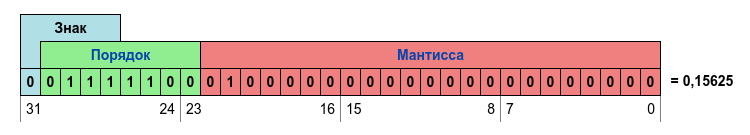
\includegraphics[width=0.9\linewidth]{\myFolder/1} \\
			Стандарт для хранения чисел с плавающей точкой. Можно почитать здесь: \href{https://ru.wikipedia.org/wiki/IEEE_754-2008}{вики}. \\
			Числа одинарной точности с плавающей запятой обеспечивают относительную точность 7-8 десятичных цифр в диапазоне от $ 10^{-38}$ до примерно $ 10^{38}$.
			Для вычисления показателя степени из восьмиразрядного поля порядка вычитается смещение порядка равное $127_{10} = 7F_{16} = 01111111_2$ (то есть, $01111100_2 - 01111111_2 = 124_{10} - 127_{10} = -3_{10}$). Так как в нормализованной двоичной мантиссе целая часть всегда равна единице, то в поле мантиссы записывается только её дробная часть. Для вычисления мантиссы к единице добавляется дробная часть мантиссы из 23-х разрядного поля дробной части мантиссы $1,01000000000000000000000_2$. Число равно произведению мантиссы со знаком на двойку в степени порядка = $1,01_2*2_{10}^{-3_{10}} = 101_2*2_{10}^{-5_{10}} = 5_{10}*2_{10}-5_{10} = 0,15625_{10}$. \\
			(Взято из \href{https://ru.wikipedia.org/wiki/%D0%A7%D0%B8%D1%81%D0%BB%D0%BE_%D0%BE%D0%B4%D0%B8%D0%BD%D0%B0%D1%80%D0%BD%D0%BE%D0%B9_%D1%82%D0%BE%D1%87%D0%BD%D0%BE%D1%81%D1%82%D0%B8}
				{другой статьи})
		\end{lecSubsection}
	\end{lecSection}
	\begin{lecSection}[Явное и неявное преобразование типов]
		\cppfile{\myFolder/2}{Неявное преобразование}{implicit_cast}
		В коде выше используется неявное преобразование: дает возможность писать код гибче, однако требует осторожнее (так, в строке 3 используется \textit{целочисленное} деление).
		\cppfile{\myFolder/3}{Не всегда удается преобразовать типы}{no_cast1}
	\end{lecSection}
	\begin{lecSection}[Типы целых чисел]
		В C++ есть несколько типов целых чисел:
		\begin{enumerate}
			\item \textbf{char} - код символа (по умолчанию 1 байт)
			\item \textbf{int} - целое число (сколько байт - не известно).
		\end{enumerate}
		Не стоит быть уверенным, что \textbf{char} - 1 байт, на разных процессорах по-разному. В C++ так устроено: язык заточен под процессор, на котором он будет выполняться. Для обоих типов можно указать \textbf{signed} и \textbf{unsigned} - знаковый тип или нет.
		\cppfile{\myFolder/sign_no_dec}{Пример доп. указателей к типам}{sign_no}. Стоит быть внимательным: сравнение для знаковых и беззнаковых может пойти не так, как хотелось бы. Пример:
		$-1 > 50$ - верное равенство, если -1 имеет тип \textbf{signed}, а 50 - \textbf{unsigned}. Проблема заключается в том, что $-1$ соответствует максимальному числу из \textbf{unsigned}.
	\end{lecSection}
	\begin{lecSection}[Логические операции]
		Работают над переменными типа \textbf{bool}.\\
		\begin{tabular}{cc}
			\multicolumn{1}{c|}{не} & $!A$ \\
			\multicolumn{1}{c|}{и} & $A\&\&B$ \\
			\multicolumn{1}{c|}{или} & $A || B$ \\
		\end{tabular}\\
		\vspace*{5pt}
		Здесь почти то же самое, что в Python, лишь синтаксис другой.
	\end{lecSection}
	\begin{lecSection}[Битовые операции C++]
		Как можно поменять две переменные без третьей? Для этого могут помочь логические операции. В C++ их несколько:
		\begin{enumerate}
			\item Инверсия -- $~x$ -- работает над \textit{любым} числом, не обязательно \textbf{bool}. Заменяет все ноли и единички в представлении числа на противоположные.
			\item Битовое \textbf{"и"} -- $x\& y$ -- умножает биты в двоичном представлении двух чисел. Иногда битовое "и" называют \textit{наложением маски}.
			\item Битовое \textbf{"или"} -- $x | y$ -- складывает биты в двоичном представлении двух чисел.
			% TODO: экранирование
			\item xor - x$\wedge$y. С его помощью можно как раз осуществить обмен переменных: \\
			x = x $\wedge$ y \\
			y = x $\wedge$ y \\
			x = x $\wedge$ y \\
		\end{enumerate}
	\end{lecSection}
	\begin{lecSection}[Автоматические типы переменных]
		\cppfile{\myFolder/auto}{Автоматический тип переменной}{auto}
		Код будет присваивать переменной х различные типы, однако этот трюк будет работать, только если компилятору сказать использовать современный стандарт (например, C++11)!
	\end{lecSection}
	
	\begin{lecSection}[Простейшие массивы]
		В C++, как и во многих языках, существуют массивы.
		\cppfile{\myFolder/array}{Пример объявления простейшего массива}{array}
		При объявлении массива надо указать его размер. По массиву можно итерироваться через обращение к элементу (точно так же, как в Питоне): A[1] -- второй элемент и так далее; нумерация идет с \textit{нуля}.\\
		 Подробнее о массивах будет рассказано на следующей лекции.
	\end{lecSection}
\end{lecture}
\stepcounter{lectureNo}

% TODO: ПОМЕНЯЙТЕ НА СВОЙ ПУТЬ ПРИ СБОРКЕ
\renewcommand{\mainFolder}{/home/aleksei/github_projects/latex_works/informatics}
\renewcommand{\myFolder}{\mainFolder/lecture_\arabic{lectureNo}/}

%	LECTURE INFO
%----------------------------------------------------------------------------------------
\renewcommand{\lectureSubject}{Адреса и указатели}
%----------------------------------------------------------------------------------------
%
% Главное - указывать в путях для добавляемых файлов переменную \myFolder.
% Так, новый cpp файл должен иметь путь \cppfile{\myFolder/main}{....} (указывается без расширения)
% Нельзя писать \cppfile{main}{...} !!!
% Если не выполнить это требование, большой проект не будет собираться


\begin{lecture}[\lectureSubject]
	\begin{lecSection}[Доступ к памяти]
		Память, выделяемая программе, неоднородна -- она делится на \textbf{сегменты}. Первый сегмент --- коды программы (режим "только чтение"). Второй -- сегмент DATA -- содержит данные программы. Более того, элементы DATA (к примеру, начальные значения переменных) записывается в .exe файл. Эти данные уходят в оперативку при запуске программы. Переменные, записанные в DATA, называются \textit{статическими}. Помимо этого, для функционирования программы необходима область \textit{стека} --- такой сегмент памяти, который заполнятся снизу вверх и изначально пуст. Когда ОС только загрузилась, в стек выделяется некоторое количество автоматической памяти -- для \textit{локальных переменных}. \\ 
		Память программе выделяется на время ее работы; после ее завершения память высвобождается.
		\cppfile{\myFolder/1}{Пример многократных вызовов функции}{1}
		Рассмотрим, как происходит работа с памятью в примере \ref{1}. Перед вызовом функции в стек программы будет выделено место для хранения "5" (оно в программе будет интерпретировано как n), stack pointer поднимается. stack pointer - это указатель, показывающий на текущее положение стека. Затем, после вызова функции, ее адрес возврата будет записан в стек - stack pointer двинется выше. Потом в стек уйдет "1" (мы же объявили ее). \\
		Попробуем написать функцию, считающую количество рекурсивных вызовов.
		\cppfile{\myFolder/2}{Функция для подсчета количества собственных вызовов}{2}
		Здесь k2 --- глобальная переменная. Ее присваивание происходит в \textit{момент компиляции} программы (т.е. она запишется в .exe и будет переноситься в память в момент загрузки). Функция \textbf{reducer} уменьшает значение k2. \\
		Однако глобальные переменные могут быть опасны! Считается, что нормальная функция не заглядывает в глобальные переменные (в таких случаях функцию называют "чистой", в противном - "грязной").
		\end{lecSection}
		\begin{lecSection}[Модификатор static]
		\cppfile{\myFolder/3}{Та же программа через static}{3}
		Мы переделали программу \ref{2}, теперь переменная k3 не видна в других блоках, но по-прежнему она записывается в сам .exe . Если бы функция была рекурсивной, то была бы такая ситуация, когда переменных k было бы много - на каждом слое рекурсии она создается. Они просто будут записаны в разные ячейки памяти и уйдут после того, как рекурсивный вызов завершится. 
		\cppfile{\myFolder/4}{Подсчет рекурсии}{4}
		В коде выше как раз \textbf{static} делает k одним для всех вызовов рекурсии --- оно при каждом вызове \underline{не} будет присваиваться в ноль. Вместо этого переменная будет увеличиваться на 1, таким образом, мы сможем увидеть глубину рекурсии.
	\end{lecSection}
	\begin{lecSection}[Указатель]
		Указатель - переменная адресного типа.
		\cppfile{\myFolder/5}{Адрес x можно указать}{5}
		Указатели тоже работают только со своими типами: в коде выше нельзя в \textbf{double*} записать число \textbf{int}. Дело в том, что возникнет ложная интерпретация -- ссылка на double превратися в ссылку на int, а поскольку в памяти double и int имеют разные размеры, то можно даже вылезти за пределы своей памяти. Компилятор это запретит, однако все можно обойти:
		\cppfile{\myFolder/6}{Пример обхода заперта}{6}
		У указателей могут тоже быть указатели:
		\cppfile{\myFolder/7}{Указатель на указатель}{7}
		Обратиться к переменной можно несколько способами:
		\cppfile{\myFolder/8}{Разница}{8}
		В последней строке происходит \textit{разыменование} адреса - грубо говоря, считывание данных из того адреса, куда указывает указатель. Разыменовывать надо последовательно:
		\cppfile{\myFolder/9}{Двойное разыменование}{9}
	\end{lecSection}
	\begin{lecSection}[Несколько слов о массивах]
		Массивов в C++ нет. Массив - это константный указатель на область памяти, представляющую содержимое!
		\cppfile{\myFolder/10}{Работа массива}{10}
		Команда объявления массива по факту означает следующее: создать n переменных типа int. \\
		С указателями можно прийти к \textit{адресной арифметике}: так, указатель $p+1$ выше означает, что мы сдвигаемся по памяти от места, куда указывает p, на \textbf{sizeof(1)}. Это иллюстрирует строка 7: A[i] абсолютно равносильна указателю *(A+i). Проверки на i \textit{нет}, то есть, в теории, мы можем убежать вообще в произвольную область памяти.
	\end{lecSection}
	\begin{lecSection}[Динамическая память]
		\cppfile{\myFolder/11}{Пример выделения из дин. памяти}{11}
		Динамическая память не является автоматической, т.е. ей надо явным образом указывать, когда ее выделять, а когда удалять. Если без конца писать вызов get(), то можно постоянно выбивать у системы память и это все приведет к \textit{memory leak} - утечке памяти.
	\end{lecSection}
	\begin{lecSection}[Передача параметров по указателю]
		Передача по параметрам бывает полезна, когда хочется поменять значение переменной внутри самой функции. Функции передается указатель и она, имея ссылку непосредственно на область памяти, может ее менять:
		\cppfile{\myFolder/12}{Передача указателей функции}{12}
		Подробнее -- в следующей лекции.
	\end{lecSection}
\end{lecture}
\stepcounter{lectureNo}

% TODO: ПОМЕНЯЙТЕ НА СВОЙ ПУТЬ ПРИ СБОРКЕ
\renewcommand{\mainFolder}{/home/aleksei/github_projects/latex_works/informatics}
\renewcommand{\myFolder}{\mainFolder/lecture_\arabic{lectureNo}/}

%	LECTURE INFO
%----------------------------------------------------------------------------------------
\renewcommand{\lectureSubject}{Динамическая память. Продолжение.}
%----------------------------------------------------------------------------------------
%
% Главное - указывать в путях для добавляемых файлов переменную \myFolder.
% Так, новый cpp файл должен иметь путь \cppfile{\myFolder/main}{....} (указывается без расширения)
% Нельзя писать \cppfile{main}{...} !!!
% Если не выполнить это требование, большой проект не будет собираться


\begin{lecture}[\lectureSubject]
	\begin{lecSection}[Динамические массивы]
		Как было сказано, массивов в C++ нет. Повторим объявление указателей: \\
		\cppfile{\myFolder/1}{Пример объявления указателей}{1}
		В строке \textbf{4} мы получаем указатель на \textbf{A[5]}. В строке \textbf{8} мы создаем число, да и еще присваиваем ему значение.
		\cppfile{\myFolder/2}{Объявление массива через \textbf{new}}{2}
		При объявлении массива через \textbf{new} нужно обязательно его удалять через \textbf{delete[]} -- оператор удаления.
	\end{lecSection}
	\begin{lecSection}[Структуры в C++]
		В C++ существует такая вещь, как структура -- набор переменных под одной крышей.
		\cppfile{\myFolder/ex1}{Простейшая структура}{ex1}
		Обратите внимание на строки \textbf{23} и \textbf{25}: такое сокращение еще часто будет встречаться (для указателей вместо "." используется "$->$"). Метод для распечатки мы вынесли отдельно для удобства. \\
		Подход к распечатке в самой первой функции имеет минус: при вызове функции мы создаем локальную копию Student. Метод \textbf{studentPrint1} лишен этого -- там передается по ссылке. Но возникает проблема, ведь мы внутри функции случайно можем изменить переменную x и этот результат будет виден извне. Решение дает передача по константной ссылке, что сделано в \textbf{studentPrint2}.\\ Существует еще одно решение задачи, в котором мы сначала создаем объект Student в памяти, получаем на него указатель, а затем через него меняем свойства объекта:
		\cppfile{\myFolder/ex2}{Еще одно решение со структурой}{ex2}
		Из структур можно составлять массивы, что неудивительно, учитывая, что массив - это просто несколько переменных. В качестве примера можно привести следующий код: \newpage
		\cppfile{\myFolder/ex3}{Массив из структур}{ex3}
	\end{lecSection}
	\begin{lecSection}[Массивы и функции]
		В функциях можно менять массивы, но их нельзя возвращать. Код внизу -- пример изменения массива внутри функции. \newpage
		\cppfile{\myFolder/ex4}{Изменение массива внутри функции}{ex4}
	\end{lecSection}
	\begin{lecSection}[Двумерный массив и передача его функции] 
		Двумерные массивы работают так же, как в Питоне. Тем не менее, у них есть некоторые особенности, связанные с их способом представления в памяти (помним, что массив по факту лишь набор переменных). Одна из этих особенностей видна в коде ниже, где мы передаем двумерный массив в функцию:
		\cppfile{\myFolder/ex5}{Передача массива в функцию}{ex5}
		Обратите внимание: в объявлении функции \textbf{printer} мы обязательно указываем длину (вторая квадратная скобка).
	\end{lecSection}
	\begin{lecSection}[Статические массивы]
		\cppfile{\myFolder/ex6}{Указание на элемент массива}{ex6}
		В коде выше видно, что для прохождения по элементам массива в функции  необходимо заранее знать его длину. Если посмотреть на выражение \ref{ex6}, то станет видно, что эта длина уходит в инструкции прохода по массиву еще на этапе компиляции, поэтому ее и нужно было передавать заранее, как это сделано в \ref{ex5}. Но можно ли сделать функцию \textbf{printer} без явного указания длины массива? Ответ дают динамические массивы.
	\end{lecSection}
	\begin{lecSection}[Динамические массивы]
		Динамические массивы --- это массивы, хранящиеся в так называемой динамической памяти (\textit{heap}). Динамические массивы объявлять несколько сложнее: так, для двумерного случая необходимо делать указатель на область памяти с указателями, каждый указатель в которой, в свою очередь, будет указывать на область памяти с нашими объектами (к примеру, \textbf{int}). Звучит не очень, однако пример \ref{ex8} может немного прояснить этот момент.
		\cppfile{\myFolder/ex7}{Объявление динамического массива}{ex7}
		\textbf{А} -- это массив из указателей типа \textbf{double*}. Каждый элемент этого массива - массив размера \textbf{width}. Таким образом, \textbf{А} есть двумерный массив. Обращение к его элементам происходит так же, как и при обычном объявлении массива, что видно в строке \textbf{26}.
		Мы сделали массив, распечатали его, а затем удалили, чтобы освободить память. При этом следует помнить такой трюк:
		\cppfile{\myFolder/ex8}{Порядок разыменования}{ex8}
	\end{lecSection}
	\begin{center}
		\tiny{В кодах лекции возможны опечатки и ошибки. Если вы найдете их, прошу сообщить \href{http://vk.com/alekseik1}{мне}.}
	\end{center}
\end{lecture}
\stepcounter{lectureNo}

% TODO: ПОМЕНЯЙТЕ НА СВОЙ ПУТЬ ПРИ СБОРКЕ
\renewcommand{\mainFolder}{/home/aleksei/github_projects/latex_works/informatics}
\renewcommand{\myFolder}{\mainFolder/lecture_\arabic{lectureNo}/}

%	LECTURE INFO
%----------------------------------------------------------------------------------------
\renewcommand{\lectureSubject}{Строки и файлы в C++}
%----------------------------------------------------------------------------------------
%
% Главное - указывать в путях для добавляемых файлов переменную \myFolder.
% Так, новый cpp файл должен иметь путь \cppfile{\myFolder/main}{....} (указывается без расширения)
% Нельзя писать \cppfile{main}{...} !!!
% Если не выполнить это требование, большой проект не будет собираться


\begin{lecture}[\lectureSubject]
	\begin{lecSection}[Хранение строк]
		Строки делятся на \textit{C-строки} и \textit{ANSI-строки}. В разных языках строки реализованы по-разному. Так, в Pascal они хранятся как \textit{ANSI-строки}: в первой ячейке памяти записана длина строки, а затем последовательно идут символы строки. Главный минус такого подхода --- ограниченность длины строки (255 символов). Этот недостаток отсутствует в \textit{C-строках}.
		
		В \textit{С-строках} используется следующая схема хранения: в памяти просто идет последовательность символов и завершается \textbf{нулем} (типа \textbf{int}, не "0"). Так, строка "Hello"\, будет записана как последовательность 'H', 'e', 'l', 'l', 'o', 0x0 (строки такого типа называются \textit{zero-ending string}). НО! Если мы сделаем обращение и изменим какой-либо символ на 0 (типа целочисленное), то строка поделится на две, ведь теперь у нее два символа окончания. Это --- один из минусов такого подхода.
	\end{lecSection}
	\begin{lecSection}[Операции со строками]
		Конкатенация строки можно делать с помощью стандартной библиотеки \textbf{cstring}.
		\cppfile{\myFolder/1}{Работа со строками}{1}
		В этом коде мы считываем строки, а затем их конкатенируем. Но Т.Ф. не любит эту библиотеку. Дело в том, что \textbf{strcat} сначала проходит и за линейное время находит ноль в конце строки, дабы узнать, где ее конец, а затем уже объединяет обе. Если такой код засунуть в цикл, то (из свойств арифметической прогрессии) мы подарим нашему коду квадратичную асимптотику.
		
		В MacOS сделано несколько интереснее: используется как число, равное длине строки, в ее начале, так и символ окончания в конце (комбинированный подход).
		
		При работе со строками следует быть осторожными: при операции \fbox{+=} можно уйти за аллоцированную (выделенную) память для данной строки и стереть ее содержимое. Кстати, в С++ строка --- это объект. Для нас сейчас это значит, что операции, которые нам кажутся простыми (наподобие \fbox{+=}), на деле такими не являются --- они реализованы по уму. К тому же, у строк есть свои методы и поля. К примеру, метод \textbf{s.size()} вернет длину строки за $O(1)$. У строк автоматическая работа с памяти --- язык автоматически выделяет столько памяти, сколько нужно.
		
		Т.Ф. рекомендует пользоваться C++ -- строками вместо С--строк.
	\end{lecSection}
	\begin{lecSection}[C++\, -- строки]
		В C++ строки входят в окружение \textbf{std}.
		\cppfile{\myFolder/2}{Объявление строки в С++}{2}
		В Python строки кодируются стандартом \underline{UTF-8}. В таком подходе память используется в разных количествах для разных символов, поэтому при вставке символа в середину строки возникают проблемы переноса (одна из причин, почему в Python строки неизменяемы). C++ лишен такого недостатка и здесь строку можно менять посимвольно.
		
		C++ не разделяет типы символа и \textit{кода} символа. Символ = код символа. Вообще, подробности можно изучить \href{http://cplusplus.com}{здесь}.
	\end{lecSection}
	
	\begin{lecSection}[Считывание строки]
		Существует несколько способов читать строки:
		\cppfile{\myFolder/3}{Считывание строки}{3}
		Обратите внимание: \textbf{cin $\gg$ s} возвращает \textbf{true} или \textbf{false}, в зависимости от того, закончился ли ввод.
		
		Другой способ заключался в методе \textbf{getline}, которому на вход поступает поток ввода (см. ниже) и строка s, куда будет записано. Различие следующее: \textbf{cin} читает до символа пробела, тогда как \textbf{getline} читает до символа переноса строки.
	\end{lecSection}
	\begin{lecSection}[Файловые потоки]
		Стандартная библиотека для работы с потоками --- это \textbf{fstream}. Она дает три потока для работы: \textbf{ifstream} для ввода и \textbf{ofstream} для вывода и \textbf{fstrim} для обоих вариантов.
		\cppfile{\myFolder/4}{Пример работы с потоками}{4}
		В коде выше было бы неплохо закрыть файл после окончания работы с ним. Более того, операционная система может дать отказ, если мы затребуем открытие слишком большого количества файлов. Однако C++ умный, он закроет файл после окончания существование объекта (в ходе выполнения деструктора, о них будет сказано в следующих лекциях).
		
		Во время открытия потока можно указать для него \textit{режим}: только для чтения и т.п.
		\cppfile{\myFolder/5}{Режимы потока}{5}
		Подробнее о режимах можно почитать в документации.
	\end{lecSection}	
	\begin{lecSection}[Строковые потоки]
		Работа со строковыми потоками тоже проходит через стандартную библиотеку:
		\cppfile{\myFolder/6}{Строковые потоки}{6}
	\end{lecSection}
	\begin{lecSection}[Односвязный список]
		Попробуем сделать односвязный список в C++ по аналогии с тем, что мы делали в Python.
		\cppfile{\myFolder/7}{Реализация односвязного списка}{7}
		\begin{enumerate}
			\item 		\textbf{typedef} --- это создание синонима типа \textbf{string}. Это сделано только для того, чтобы не писать каждый раз \textbf{std::string}, другого назначения у такой конструкции для нас нет.
			\item \textbf{struct tNode} --- объявление структуры ноды. В ней всего две переменные: свое значение и ссылка на следующую ноду.
			\item \textbf{tNode * \dots} --- сигнатура функции \textit{insert}\_\textit{node}. Ее мы опишем позже.
			\item В методе \textbf{main} мы создаем ноду через \textbf{new}, затем сохраняем ссылку на созданный объект. После этого мы записываем туда какую-то информацию ("Hello" в примере), далее прикрепляем к ней другие ноды.
			\item В цикле мы прогуливаемся по всем нодам и выводим их содержимое. Обратите внимание на переход к следующей ноде в последней строке цикла.
			\item Функция \textbf{insert\_node} --- изюминка нашего кода. Ей передается указатель на нашу ноду. Внутри функции мы создаем новую ноду, заполняем в нее данные из \textbf{data}, а в качестве следующей ноды записываем ту, что мы передали функции. Из этого получается, что мы добавляем ноды в обратном порядке, так как только что созданная нода встает впереди старой.
		\end{enumerate}
	\end{lecSection}
\end{lecture}
\stepcounter{lectureNo}

